\chapter{Requirement Analysis and Concept}
\label{ch:chapter03}
Alice, Bob and Carol want to trade assets they own on different blockchains. Since they do not trust each other they need a solution where the trade is either executed completely or reversed. They want their assets to be returned in case a party behaves irrationally. For example if Carol tries to scam them, Alice and Bob do not want to loose their assets and end up worse in the swap process. The example \ref{subsec:background:second_section:example} discussed in chapter model and general principles \ref{ch:background} is the user story that is addressed by the prototype implementation. Requirements to implement a system feasible of solving their initial situation in an atomic matter is discussed next. First the blockchain needs to support turing-complete smart contracts to hold information during the trade and to decide weather the swap contract is unlocked or timed out. By holding these information the contract can decide if the locked funds are eligible to be claimed by the counter party or if the party can claim a refund in case the contract is timed out. Second is a digraph implementation as a smart contract to execute the swap decentralized. For simplicity delegation can be handled by the middleware, by splitting the trade into two phases that are discussed in chapter \ref{ch:chapter04}. Third requirements are the hashlocks and timelocks. The correct hashlock is needed to unlock the contract by appending it to the secret revealed by the party leading the digraph paths. To unlock the contract before it times out timelocks passed to the unlock function need to be smaller than the prematurely added timelocks that are held by the contract state. If the unlock limits are surpassed the contract times out and allows the party which locked their funds on contract creation to reclaim them. For full decentralization the hashlocks and timelocks need to be created by the smart contract, but for simplicity the middleware creates them. By passing the values to the smart contract's claim and refund functions as parameter it can decide if the phases are completed in the correct time windows or if the trade is canceled. The UML use case diagram \ref{fig:uml_use_case} below shows interactions between the actors and systems. In a productive environment the participating parties would be outside the system, but again for simplicity the implemented prototype handles all steps of the actors to complete the swap. The implementation chapter \ref{ch:chapter04} discuss the realization of the use case diagram in detail. Including an UML class diagram and abstraction of the swap digraph.


%TODO MB add sequence diagram!!

\begin{figure}[h]
	\begin{center}
		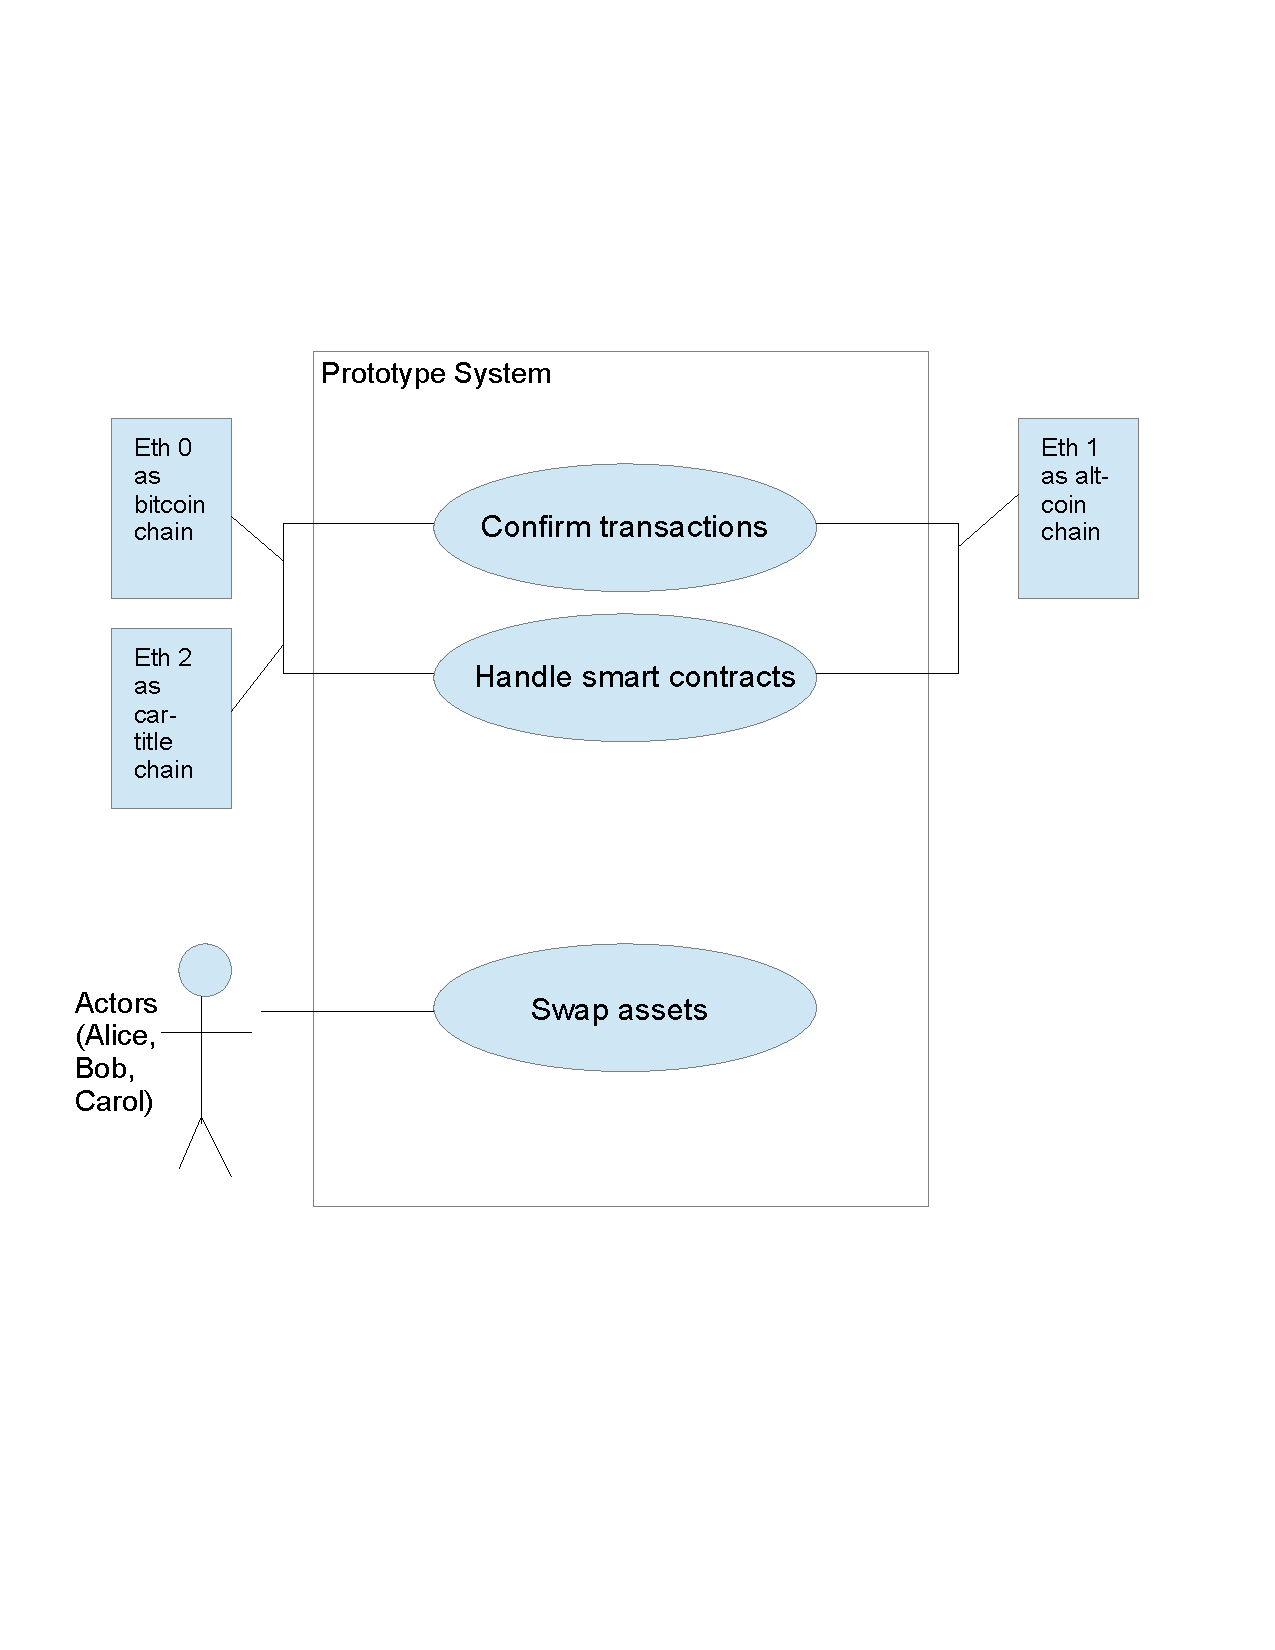
\includegraphics[width=0.7\paperwidth]{uml}	
		\caption{UML Use Case Diagram}
		\label{fig:uml_use_case}
	\end{center}
\end{figure}


\chapter{Implementation}
\label{ch:chapter04}
The prototype presented in this chapter aims to implement the three-way swap example of Alice, Bob and Carol discussed earlier in chapter \ref{subsec:background:second_section:example}. Implementing the protocol from chapter \ref{subsec:background:second_section:protocol} to execute any kind of swap would be too much work for this thesis. For simplicity this work uses three ethereum blockchains posing as the bitcoin, alt-coin and car-title blockchain. All communication with the blockchains is handled through the Geth client \cite{gethclient}. Also for simplicity certain parts of Herlihy's proposed smart contracts are executed off-chain, such as the generation of the hashlock and timelock values and it's verification. The prototype utilitizes class Pools, which holds a wallet one each chain containing ethereum accounts with mined ether to prepare the initial situation of Alice, Bob and Carol. The Pools class also serves another purpose, due to a problem that came up during the implementation. Ether moved by a smart contract are executed as internal transactions, which are only held by the state of the \ac{EVM}'s stack and thus are not visible on an account's balance. To overcome this issue the class Pools sends one ether upon a successful call of the claim() function of the corresponding smart contract to the callers's account, to make the transfer visible during run time. There are methods to trace internal transactions of a smart contract by instrumenting the \ac{EVM} \cite{instrumentingEVM}, which is discussed in chapter \ref{sec:background:futureresearch}. In order to delegate the actions made by the participating parties a java middleware is needed, which implements the wallets and communicates with the blockchains through the geth clients. It also prepares the initial situation for the parties mentioned in the example by controlling the pool accounts to distribute assets to the participating parties. Classes Alice, Bob and Carol represent the parties and have control of their assets in order to send ether and deploy contracts. The middleware uses the web3j library \cite{web3j} to communicate with the geth clients. The class HashLock generates hashlock $h$ with the given formula $h$ = $H$($s$), where $H$($\cdot$) is a cryptographic hash function using the \ac{SHA-256} hashing algorithm. It takes the secret $s$ with the appended current block and resolves to the hashed secret $s$ (hashlock $h$), which can be reached only with the correct secret and block. Smart contracts can determine the current time only by the system state, meaning the contracts can only measure time by the current block number in the blockchain e.g. block \# 10 is later than block \# 5. To measure a real time like \ac{UTC} the implementation still needs to be off-chain with a corresponding time server. Class TimeLock generates start times and holds information and saves them into the published smart contract, when phases have to be completed in order to execute the swap protocol. The middleware needs a smart contract solidity file, so all parties can deploy and publish the contract onto the blockchains. Class Digraph delegates the swap protocol for the parties. Instances Alice, Bob and Carol representing the actors are passed to Digraph's constructor upon initialization. Paths are triggered by instance Digrap by the according string representations (table \ref{table:2}), which then call the functions in a given order and executes the swap in behalf of Alice, Bob and Carol. The swap is executed in two phases, called Phase 0 (contract deployment and locking of funds figure \ref{fig:phase0}) and 1 (revealing secrets figure \ref{fig:phase1}). \newline

\begin{table}[h!]
	\centering
	\begin{tabular}{|c | c | c |} 
		\hline 
		\textcircled{1} & String s = "AB" & Alice deploys on alt-coin chain\\ [0.5ex] 
		\hline
		\textcircled{2} & String s = "BA" & Bob deploys on bitcoin chain\\ 
		\hline
		\textcircled{3} & String s = "CC" & Carol deploys on car-title chain \\
		\hline
		\textcircled{4} & String s = "AC" & Alice unlocks Carol's contract and claims car-title \\ [1ex] 
		\hline
		\textcircled{5} & String s = "CA" & Carol unlocks Bob's contract and claims bitcoin \\ [1ex] 
		\hline
		\textcircled{6} & String s = "BB" & Bob unlocks Alice's contract and claims alt-coin \\ [1ex] 
		\hline
	\end{tabular}
	\caption{Digraph Path String Representations}
	\label{table:2}
\end{table}

\begin{figure}[h]
	\begin{center}
		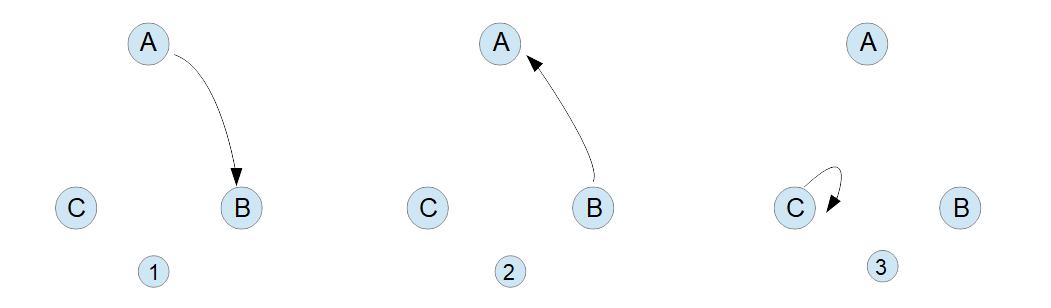
\includegraphics[width=0.6\paperwidth]{phase0}	
		\caption{Swap Protocol Phase 0}
		\label{fig:phase0}
	\end{center}
\end{figure}

\begin{figure}[h]
	\begin{center}
		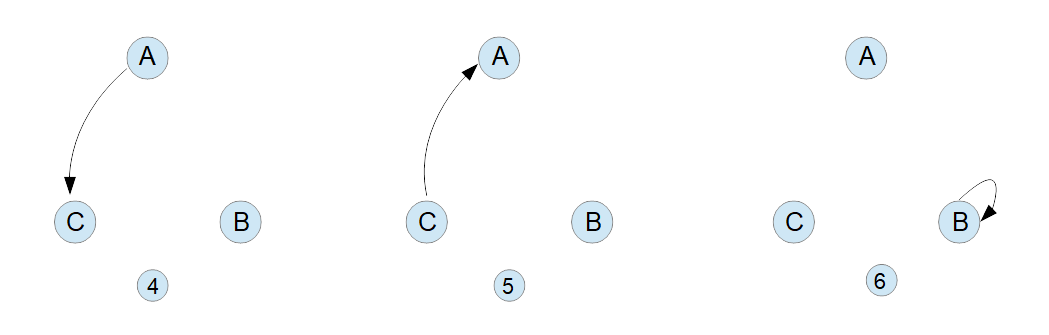
\includegraphics[width=0.6\paperwidth]{phase1}
		\caption{Swap Protocol Phase 1}
		\label{fig:phase1}
	\end{center}
\end{figure}

\clearpage


\section{Reference Architecture}
\label{sec:chapter04:ref_architecture}

This chapter discusses the reference architecture (figure \ref{fig:reference_architecture}) resulting from the swap prototype implementation. Alice, Bob and Carol are the actors and represent any user in a productive environment. In the swap prototype implementation actors are controlled and delegated by the middleware, in the case of the reference architecture actors would be real users though and each of them would be responsible to stick to the swap protocol by themselves. This includes the two phases, meaning actors have to deploy contracts and send funds in the correct order, as well as revealing the secret and claiming the traded funds. If any of the the actors do not apply to the protocol, the swap is canceled and funds are returned to the actors so no party ends up worse in the case of malicious behavior. The java middleware implements the web3j library to communicate with the ethereum geth clients, which then handle all interactions with the blockchains. In a real productive environment the three ethereum chains can be swapped with any blockchain that supports smart contracts and turing-completeness. Implementation of additional libraries to communicate with the corresponding blockchain is needed. The reference architecture shown below can be used as foundation for universal swap systems to support any kind of swap. To get an architecture for a two-way swap this can easily be done by detaching actor 2 and chain 2 from the reference architecture for example. \newline \newline

%TODO MB write 2 more sentences!!

\begin{figure}[h]
	\begin{center}
		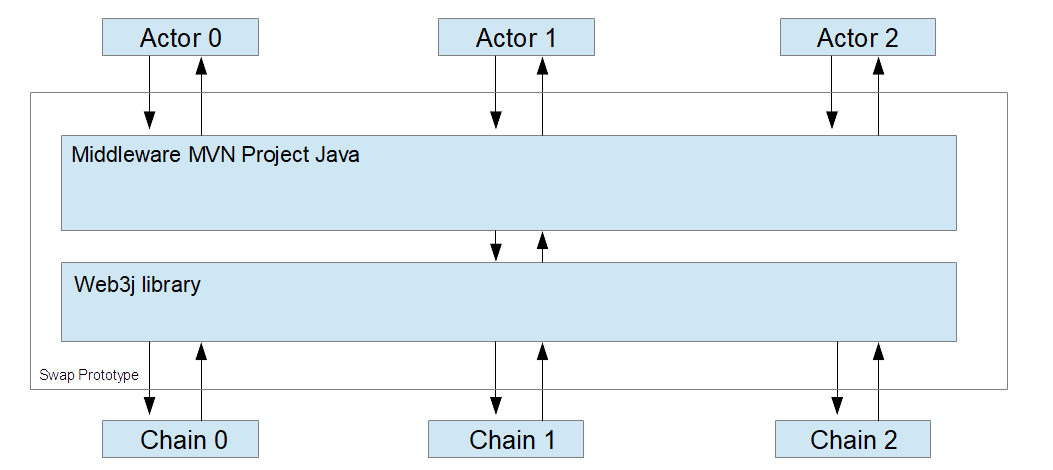
\includegraphics[width=0.6\paperwidth]{reference_architecture}
		\caption{Swap Protocol Reference Architecture}
		\label{fig:reference_architecture}
	\end{center}
\end{figure}
\clearpage

%
% Section: Listen
%
\section{Swap Contract}
\label{sec:chapter04:smartcontracts}

The swap contract (figure \ref{fig:swap_contract}) holds several attributes (line 4 - 9) to force correct execution of the swap protocol, which are passed to the constructor (line 11 - 21) upon initialization. The contract holds the addresses of the party and counter party. The contract is always deployed by each actor on the blockchain he owns the assets to be traded in the swap process. The timelock and start values are saved in the swap contract's state to ensure that the participating parties stick to the protocol. With these attributes the swap contract can decide if assets are eligible either for a claim or refund. The hashlock attribute ensures that funds can only be claimed by unlocking all values in the unlocked bool array. To unlock the entries in the array the counter party needs the correct revealed and hashed secret. Each entry of the unlocked array is initialized false during initialization by the swap contract constructor. The unlock function (line 24 - 29) can only be called by the counter party, which was saved in the swap contract's state upon initialization. Entries in the unlocked array are only set to true by passing the correct hashlock and time. If the timeNow value passed to the function is greater than the saved timelock value in the contract's state, then the unlocked entry is not set to true and prevents the funds being claimed by the counter party. The isUnlocked function (line 32 - 34) returns the bool value of the unlocked array for the passed function's argument entry i. The lockEther function (line 36 - 38) is called by the party after successful deployment of the swap contract to lock the funds offered for trade in the contract. The refund function (line 40 - 46) takes timeNow as an argument and can only be called contract's owner or party that deployed the swap contract. If timeNow value is greater than the last entry in the timelock array, then the funds are returned to the contract's owner and the trade is canceled. The claim function (line 48 - 53) can only be called by the counter party saved in the swap contract's state upon initialization. Funds are only released to the counter party, if all entries in the unlocked array are set to true. In the case of Alice, Bob and Carol each party deploys its own contract on the blockchain they offer funds to be swapped in the process of protocol execution. The contract shown below is written in solidity and is only compatible with ethereum blockchains, but the code logic can be transferred to any other blockchain that supports smart contracts to execute swaps between other types of blockchains.


\begin{figure}[h]
	\begin{center}
		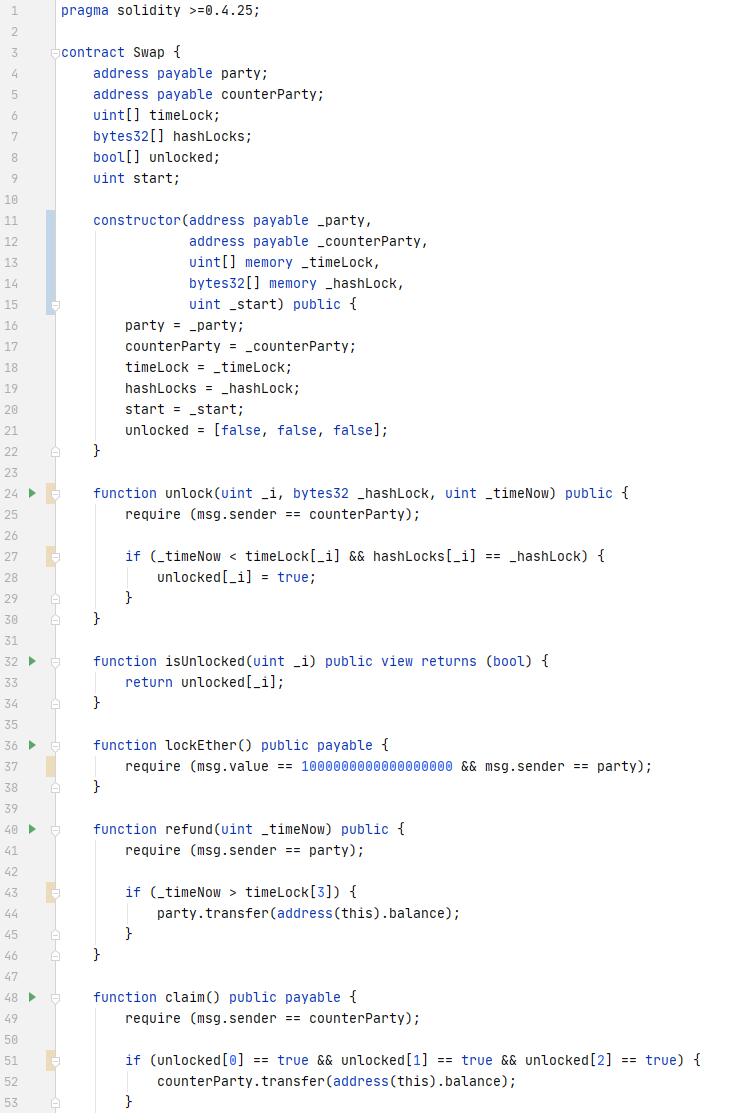
\includegraphics[width=0.7\paperwidth]{swap_contract}
		\caption{Swap Contract}
		\label{fig:swap_contract}
	\end{center}
\end{figure}
\clearpage

\section{Middleware (Intermediate Party)}
\label{sec:chapter04:middleware}

This chapter discusses the middleware of the swap prototype, it's classes and shows an UML diagram (figure \ref{fig:uml}) on the next page. Class EthNode holds information for each ethereum node like the name, host and port. These values are needed to for initialization of the Web3j object, which handles the communication with the geth clients to interact with the blockchains. Class Wallet retrieves the Web3j object from the EthNode class it wants to interact with. The Wallet class wraps all functions of the Web3j library that are needed to execute the swap protocol and implements an API that can be extended with other libraries to support different blockchains. The current implementation of the swap prototype only supports ethereum chains though. Class Pools is a helper to prepare the initial swap situation of Alice, Bob and Carol. It holds wallets on each of the three blockchains with enough funds to supply the participating parties with the assets they intend to swap during runtime. The class is also used to make the internal transactions of the smart contracts visible on the balance by sending additional funds. Class HachLock generates the hashlock $h$ with the secret $s$ which is passed to the constructor when instantiated. By calling the function getHashLockAsByteArrayWithCurrentBlockAppended and passing the current block as function's argument, it digests the hashlock $h$ as a byte array. Class TimeLock is instantiated with the current time and the time values, which determine the window for completion of the phases 0 and 1. It generates all Date values to enforce that each contract receives the correct times in which the swap phases have to be executed. The Digraph class delegates the swap protocol for the participating parties. It triggers the paths one after another in  the correct order and handles all actions of Alice, Bob and Carol to fully execute the swap. Package Parties holds the classes Alice, Bob and Carol and has full control over their assets. In a productive environment these classes would be real users and the actor classes could be abandoned from the swap prototype. Class SwapProtocol instantiates the classes Alice, Bob, Carol and Digraph. The parties hold their private keys as attributes and connect to their nodes during initialization, when al parties are ready and the initial trade situation is prepared the class Digraph triggers the paths in the correct order to execute the swap protocol. A simple console interface is provided by the class App, where the user can choose between running different tests or execute a three-way swap. For simplicity hashlock $h$, timelock $t$ and digraph $D$ are generated off-chain by their corresponding classes.

\begin{figure}[h]
	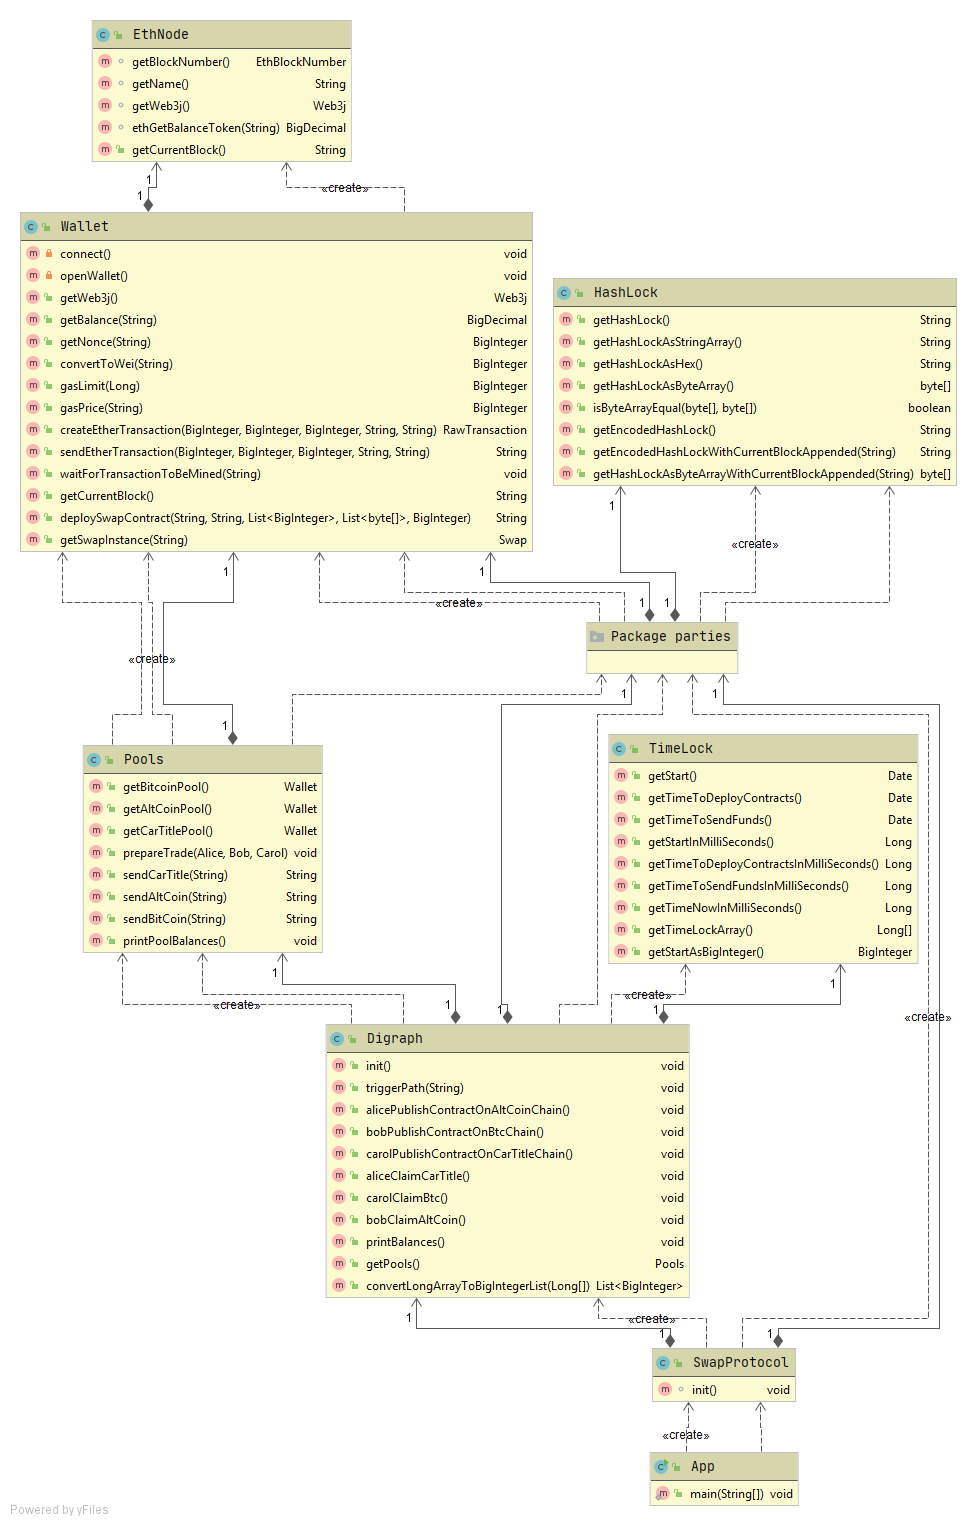
\includegraphics[width=0.7\paperwidth]{swaps-crop}
	\caption{UML Class Diagram Middleware}
	\label{fig:uml}
\end{figure}
\clearpage

\section{Tests (Evaluation)}
\label{sec:chapter04:poc}
Testing is difficult due to a problem that came up during implementation of the swap prototype. The \ac{EVM} handles funds sent by a smart contract as internal transactions, which do not show up on the recipients account balance. Information who owns the coins after sending it is only available in the contract's state. Making them visible requires tracing the \ac{EVM}'s stack on assembly level to keep track on who owns the funds. The prototype implementation uses a workaround to simulate the result of a claim or refund function call of the swap contract. It does that by sending funds from one of the pool accounts to the caller's address to make the transaction visible on the balance. This influences execution times of the prototype and test results. Since three chains and the prototype are all running on the same system, test results do not represent a productive environment. To reproduce the testing results an equivalent system is required, where the swap prototype and chains are hosted on. Nevertheless test results of the implemented system are discussed next. Swaps per hour (SPH) is calculated by measuring the time one swap needs to complete. One run includes preparation of the Alice, Bob and Carol's initial situation, connecting to wallets and the workaround discussed above. The values shown by table \ref{table:3} result in approximately eight swaps per hour by dividing one hour in nanoseconds through the average time of the three runs. Transactions per second (TPS) are measured by sending ten transaction and measure the time they need until transactions are published and confirmed on the blockchain. By dividing ten through the average time in seconds of table \ref{table:4} the transactions per second on one chain is approximately 0.049 TPS.

\begin{table}[h!]
	\centering
	\begin{tabular}{|c | c | c |} 
		\hline 
		Iteration & Time in nanoseconds & Time in minutes \\ [0.5ex] 
		\hline \hline
		Run 1 & 377392865700 ns & 6.29 min  \\ 
		\hline
		Run 2 & 435784403900 ns & 7.26 min  \\
		\hline
		Run 3 & 423182624900 ns & 7.05 min  \\
		\hline
		Average & 412119964833 ns & 6.87 min  \\ [1ex] 
		\hline
	\end{tabular}
	\caption{Test results swaps per hour (SPH)}
	\label{table:3}
\end{table}

\begin{table}[h!]
	\centering
	\begin{tabular}{|c | c | c |} 
		\hline 
		Iteration & Time in nanoseconds & Time in seconds \\ [0.5ex] 
		\hline \hline
		Run 1 & 56932675400 ns & 56.93 sec  \\ 
		\hline
		Run 2 & 55702292100 ns & 55.70 sec  \\
		\hline
		Run 3 & 71745206200 ns & 71.75 sec  \\
		\hline
		Average & 61460057900 ns & 61.46 sec  \\ [1ex] 
		\hline
	\end{tabular}
	\caption{Test results transactions per second (TPS)}
	\label{table:4}
\end{table}

\chapter{Conclusion and Future Research}
\label{ch:chapter05}
The atomic cross-chain prototype discussed in chapter \ref{ch:chapter04} shows that swapping assets across different is possible with the use of smart contracts. To reach full decentralized blockhain interoperability more needs to be done though. For simplicity the prototype handles delegation of the trade and generation of the hashlocks and timelocks off-chain. By adding these features as smart contract implementations the prototype can be further decentralized. It remains an open question if bitcoin can implement swaps with the current scripting language it supports, because the lack of turing-completeness is a problem. To implement and generate the timelocks on-chain there needs to be evaluation on how time can be measured in block generation times, because the \ac{EVM} only knows time by the current world state and past blocks that have been added. Hyperledger implements their approach with Hashed-Timelock Agreements \cite{HTLAs}, which are based on the timelock \cite{timelock} principle of bitcoin. After successful decentralization of delegation and generation of timelocks and hashlocks on-chain next step is supporting other cryptocurrencies that support smart contracts. Further evaluation is needed to see if different consensus algorithms bring up more problems to be solved for executing swaps. A list of cryptocurrencies that have smart contract support created by cryptoslate \cite{smart_contract_coins} shows that it needs a lot more research on this topic to reach full interoperability of these blockchains. Before even adding support for other cryptocurrencies to the prototype further development of ethereum's clients and libraries has to be done to make internal transactions visible to the end user by instrumenting the \ac{EVM} \cite{instrumenting_evm}. Also the prototype does not support two-way swaps of assets between two chains at this time. Solving the previous mentioned tasks and the problems that come up during further evaluation of these, the next logical step is to support more cryptocurrencies to create a framework that supports any kind blockchain technologies.

%TODO: MB add two more sentences!!

\chapter{Terminology}
\label{ch:chapter06}

\begin{center}
	\begin{tabular}{ p{4cm} p{8cm} } 
		Address: & A 160-bit code used for identifying Accounts.  \\ 
		Account: & Accounts have an intrinsic balance and transaction count held as part of ethereum state. Those accounts with empty associated \ac{EVM} code are controlled by external entities and those with non-empty \ac{EVM} code (thus the account represents an autonomous object). Every Account has a single address that identifies it. \\
		Alt-Coin: & The term Alt-Coin refers to all cryptocurrencies launched after the success of bitcoin. Generally, they sell themselves as better alternatives to bitcoin or try to solve certain technological problems in a "better" or different way. \\
		App: & An app is a type of software that allows you to perform specific tasks. Its also an acronym for application. Its often named after the device the application is running on. E.g. mobile app, desktop app or \ac{DApp}. Decentralized apps are a referral for applications running on decentralized architectures like the \ac{EVM}. \\
		Asset: & An asset is a resource with economic value, owned or controlled by an individual, corporation or country. In financial context it comes with the expectation that it provides a future benefit. In context of this work it can also be a car title owned by an individual like Carol.\\
		Atomic Transaction: & Atomic Transactions are associated with Database operations where a set of actions must all complete or else none of them complete (atomicity). Same concept applies to swaps in blockchain context. \\
		Autonomous Object: & A notional object, which is existent only in the hypothetical state of the ethereum public chain. It has an address and thus an associated account, which has non-empty \ac{EVM} code. Incorporated only as the Storage State of that account. \\
	\end{tabular}
\end{center}

%  App:  -> According to Wood an app is the end-user-visible application hosted in the ethereum browser.

\clearpage

\begin{center}
	\begin{tabular}{ p{4cm} p{8cm} }
		Block: & A block is a set of transactions, smart contracts and meta data, appended to the previous block in the blockchain. It has to be verified (mined) by the nodes of the network to become valid. \\
		Block Time: & It defines the time that it takes for a block to get confirmed (mined) by participants of the network. In case of ethereum there is an expected block time of 10 to 19 seconds. \\
		Bytecode: & Bytecode is the language which the \ac{EVM} understands and can execute. Smart contracts are often written in a high level programming language like solidity and compiled down to bytecode, which consists of a series of bytes, where each byte represents an operation for the \ac{EVM} to execute. Its often referred to as \ac{EVM Code}. \\
		Cryptocurrency: & A cryptocurrency is a digital asset designed to work as medium of exchange and most of the time not issued by any state or central bank. The individual coin ownership are stored in a ledger, using strong cryptography to secure transaction records, to control the creation of additional coins, and to verify the transfer of coin ownership. \\
		CryptoNote: & CryptoNote is an application layer protocol which aims to solve specific problems of bitcoin. These are respectively traceability of transactions, the \ac{PoW} function, irregular emission, hardcoded constants and bulky scripts. The protocol is the basis of several decentralized privacy-oriented cryptocurrencies. \\
		Contract:  & Generally a contract is a written or spoken agreement, especially one concerning employment, sales, or tenancy, that is intended to be enforceable by law. In ethereum or cryptocurrency environment a contract is more meant to be a financial contract and mostly referred to as smart contract. \\
		External Actor: & An external actor in the context of this thesis is an entity, which resides and acts outside or inside of the cryptocurrency system, with potential malicious behavior. \\
	\end{tabular}
\end{center}

\clearpage

\begin{center}
	\begin{tabular}{ p{4cm} p{8cm} } 
		Ether: & Ether (short ETH) is the internal cryptocurrency of the ethereum blockchain. It can be transferred from account to account, but is also used to pay the gas fees for smart contracts and their execution of functions. \\
		Ethereum Virtual Machine: & Ethereum provides a decentralized virtual machine, called the \ac{EVM}. It can execute scripts by using an international network of public nodes, in case of the ethereum public chain. The virtual machine's instruction set is Turing-complete. \\
		Gas: & Its the fundamental network cost unit and can be converted freely from and to Ether as required. Gas does not exist outside of the computational engine of ethereum, its price is set by the transactions. Miners are free to ignore transactions, which have a too low gas price. \\
		Genesis Block: & The genesis block is the first ever mined or origin block of a public or private ethereum network. It contains all essential information to configure the network and as well how to find related peers. \\
		Hash: & Is the result of any hash function that can be used to map data of arbitrary size to fixed-size values. The values returned by a hash function are always the same result of same input and are called hash values, hash codes, digests or simply hashes. \\
		Padding: & All six SHA functions (SHA-0, SHA-1, SHA-224, SHA-256, SHA-384 and SHA-512) start by padding the message according to the so-called Merkle-Damg{\aa}rd strengthening technique. The message is appended with a binary one and right-padded with a variable number of zeros, followed by the length of the original message coded over two binary words. The total padded message length must be a multiple of the message block size of the according function. \\
	\end{tabular}
\end{center}

\clearpage

\begin{center}
	\begin{tabular}{ p{4cm} p{8cm} }
		Protocol: & Generally a protocol is a system of rules how a computer and its developers can connect to, participate in and transmit information over a system or network. These instructions define code syntax and semantics that the system expects. Ethereum's protocol is built and designed for decentralized applications, with emphasis on rapid development time, security and interactivity. \\
		Public Key: & In ethereum context the public key is derived from the private key using \ac{ECDSA}. Its also a synonym for the address.  \\
		Public Blockchain: & A public blockchain is a distributed and decentralized open network. Anyone can download the protocol and read, write or participate in it. Transactions are recorded as blocks and linked together to form a chain. \\
		Private Key: & A private key is a large random number, which is also used to create the public key or address. The private key allows the user to sign and send transactions. Whoever owns the private key has full control over the ether associated with the account. \\
		Private Blockchain: & A private blockchain is a completely private blockchain, which is isolated from other public blockchains. Private chains are mainly created by organizations to restrict the read and write permissions, only nodes with the right permissions can access these blockchains. \\
		Storage State: & Storage state is the information particular to a given account, which is maintained between the times that an account runs associated \ac{EVM Code}. \\
		Solidity: & Solidity is a high-level and object-oriented programming language for implementing smart contracts. The code gets compiled down to bytecode for the ethereum blockchain to execute. \\
	\end{tabular}
\end{center}

\clearpage

\begin{center}
	\begin{tabular}{ p{4cm} p{8cm} }
		Transaction:  & A transaction in ethereum context is the way an external actor interacts with the ethereum network, if someone wants to modify or update the state stored in the blockchain. \\
		Token: & Ethereum tokens are simply digital assets, which are being built on top of the ethereum blockchain. They can also strengthen ethereum's ecosystem, since ether are needed to execute the smart contracts on which the tokens a built on. \\
		Miner: & The process in which transactions are verified and added to the blockchain digital ledger is called cryptocurrency mining. The external actor or entity that runs the node in the network is called a miner. \\
		Nonce: & The nonce is the number of transactions sent from a given address, each time a transaction is sent from a given account the nonce is increased by one. Its specific value before and after increasing can only be used once. \\
		On-chain: & An on-chain transaction (synonym for transaction), occurs and is considered valid when the blockchain is modified to reflect the transaction on the public ledger. Smart contracts and all pieces of code, that get executed by the \ac{EVM} for example are considered to be on-chain. \\
		Off-chain: & An off-chain transaction takes the value outside of the blockchain. It can be executed using multiple methods and patterns. Off-chain implementations are all kinds of software, which takes some part in transaction or data verification off the blockchain. \\
	\end{tabular}
\end{center}


% internal transaction



